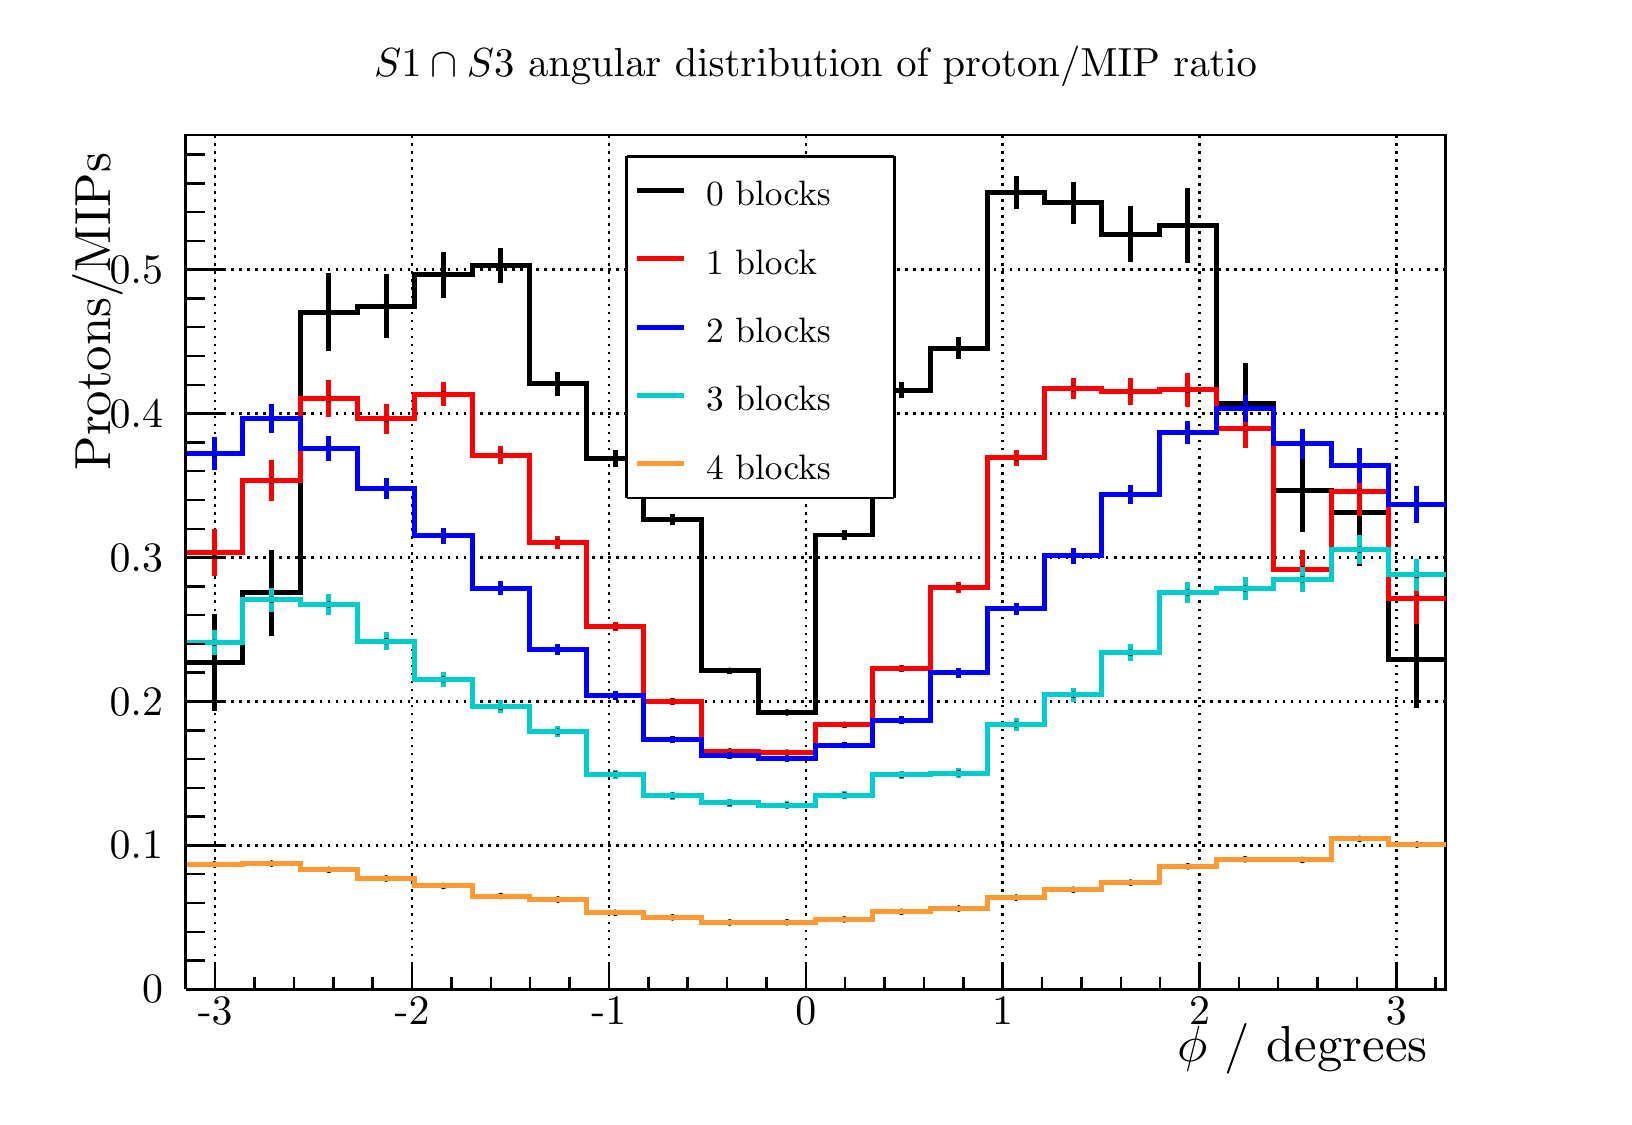
\begin{tikzpicture}
\pgfdeclareplotmark{cross} {
\pgfpathmoveto{\pgfpoint{-0.3\pgfplotmarksize}{\pgfplotmarksize}}
\pgfpathlineto{\pgfpoint{+0.3\pgfplotmarksize}{\pgfplotmarksize}}
\pgfpathlineto{\pgfpoint{+0.3\pgfplotmarksize}{0.3\pgfplotmarksize}}
\pgfpathlineto{\pgfpoint{+1\pgfplotmarksize}{0.3\pgfplotmarksize}}
\pgfpathlineto{\pgfpoint{+1\pgfplotmarksize}{-0.3\pgfplotmarksize}}
\pgfpathlineto{\pgfpoint{+0.3\pgfplotmarksize}{-0.3\pgfplotmarksize}}
\pgfpathlineto{\pgfpoint{+0.3\pgfplotmarksize}{-1.\pgfplotmarksize}}
\pgfpathlineto{\pgfpoint{-0.3\pgfplotmarksize}{-1.\pgfplotmarksize}}
\pgfpathlineto{\pgfpoint{-0.3\pgfplotmarksize}{-0.3\pgfplotmarksize}}
\pgfpathlineto{\pgfpoint{-1.\pgfplotmarksize}{-0.3\pgfplotmarksize}}
\pgfpathlineto{\pgfpoint{-1.\pgfplotmarksize}{0.3\pgfplotmarksize}}
\pgfpathlineto{\pgfpoint{-0.3\pgfplotmarksize}{0.3\pgfplotmarksize}}
\pgfpathclose
\pgfusepathqstroke
}
\pgfdeclareplotmark{cross*} {
\pgfpathmoveto{\pgfpoint{-0.3\pgfplotmarksize}{\pgfplotmarksize}}
\pgfpathlineto{\pgfpoint{+0.3\pgfplotmarksize}{\pgfplotmarksize}}
\pgfpathlineto{\pgfpoint{+0.3\pgfplotmarksize}{0.3\pgfplotmarksize}}
\pgfpathlineto{\pgfpoint{+1\pgfplotmarksize}{0.3\pgfplotmarksize}}
\pgfpathlineto{\pgfpoint{+1\pgfplotmarksize}{-0.3\pgfplotmarksize}}
\pgfpathlineto{\pgfpoint{+0.3\pgfplotmarksize}{-0.3\pgfplotmarksize}}
\pgfpathlineto{\pgfpoint{+0.3\pgfplotmarksize}{-1.\pgfplotmarksize}}
\pgfpathlineto{\pgfpoint{-0.3\pgfplotmarksize}{-1.\pgfplotmarksize}}
\pgfpathlineto{\pgfpoint{-0.3\pgfplotmarksize}{-0.3\pgfplotmarksize}}
\pgfpathlineto{\pgfpoint{-1.\pgfplotmarksize}{-0.3\pgfplotmarksize}}
\pgfpathlineto{\pgfpoint{-1.\pgfplotmarksize}{0.3\pgfplotmarksize}}
\pgfpathlineto{\pgfpoint{-0.3\pgfplotmarksize}{0.3\pgfplotmarksize}}
\pgfpathclose
\pgfusepathqfillstroke
}
\pgfdeclareplotmark{newstar} {
\pgfpathmoveto{\pgfqpoint{0pt}{\pgfplotmarksize}}
\pgfpathlineto{\pgfqpointpolar{44}{0.5\pgfplotmarksize}}
\pgfpathlineto{\pgfqpointpolar{18}{\pgfplotmarksize}}
\pgfpathlineto{\pgfqpointpolar{-20}{0.5\pgfplotmarksize}}
\pgfpathlineto{\pgfqpointpolar{-54}{\pgfplotmarksize}}
\pgfpathlineto{\pgfqpointpolar{-90}{0.5\pgfplotmarksize}}
\pgfpathlineto{\pgfqpointpolar{234}{\pgfplotmarksize}}
\pgfpathlineto{\pgfqpointpolar{198}{0.5\pgfplotmarksize}}
\pgfpathlineto{\pgfqpointpolar{162}{\pgfplotmarksize}}
\pgfpathlineto{\pgfqpointpolar{134}{0.5\pgfplotmarksize}}
\pgfpathclose
\pgfusepathqstroke
}
\pgfdeclareplotmark{newstar*} {
\pgfpathmoveto{\pgfqpoint{0pt}{\pgfplotmarksize}}
\pgfpathlineto{\pgfqpointpolar{44}{0.5\pgfplotmarksize}}
\pgfpathlineto{\pgfqpointpolar{18}{\pgfplotmarksize}}
\pgfpathlineto{\pgfqpointpolar{-20}{0.5\pgfplotmarksize}}
\pgfpathlineto{\pgfqpointpolar{-54}{\pgfplotmarksize}}
\pgfpathlineto{\pgfqpointpolar{-90}{0.5\pgfplotmarksize}}
\pgfpathlineto{\pgfqpointpolar{234}{\pgfplotmarksize}}
\pgfpathlineto{\pgfqpointpolar{198}{0.5\pgfplotmarksize}}
\pgfpathlineto{\pgfqpointpolar{162}{\pgfplotmarksize}}
\pgfpathlineto{\pgfqpointpolar{134}{0.5\pgfplotmarksize}}
\pgfpathclose
\pgfusepathqfillstroke
}
\definecolor{c}{rgb}{1,1,1};
\draw [color=c, fill=c] (0,0) rectangle (20,13.5632);
\draw [color=c, fill=c] (2,1.35632) rectangle (18,12.2069);
\definecolor{c}{rgb}{0,0,0};
\draw [c,line width=0.9] (2,1.35632) -- (2,12.2069) -- (18,12.2069) -- (18,1.35632) -- (2,1.35632);
\definecolor{c}{rgb}{1,1,1};
\draw [color=c, fill=c] (2,1.35632) rectangle (18,12.2069);
\definecolor{c}{rgb}{0,0,0};
\draw [c,line width=0.9] (2,1.35632) -- (2,12.2069) -- (18,12.2069) -- (18,1.35632) -- (2,1.35632);
\draw [c,line width=0.9] (2,1.35632) -- (18,1.35632);
\draw [c,dotted,line width=0.9] (2.375,12.2069) -- (2.375,1.35632);
\draw [c,dotted,line width=0.9] (4.875,12.2069) -- (4.875,1.35632);
\draw [c,dotted,line width=0.9] (7.375,12.2069) -- (7.375,1.35632);
\draw [c,dotted,line width=0.9] (9.875,12.2069) -- (9.875,1.35632);
\draw [c,dotted,line width=0.9] (12.375,12.2069) -- (12.375,1.35632);
\draw [c,dotted,line width=0.9] (14.875,12.2069) -- (14.875,1.35632);
\draw [c,dotted,line width=0.9] (17.375,12.2069) -- (17.375,1.35632);
\draw [c,dotted,line width=0.9] (2.375,12.2069) -- (2.375,1.35632);
\draw [c,dotted,line width=0.9] (17.375,12.2069) -- (17.375,1.35632);
\draw [c,line width=0.9] (2,1.35632) -- (2,12.2069);
\draw [c,dotted,line width=0.9] (18,1.35632) -- (2,1.35632);
\draw [c,dotted,line width=0.9] (18,3.18443) -- (2,3.18443);
\draw [c,dotted,line width=0.9] (18,5.01255) -- (2,5.01255);
\draw [c,dotted,line width=0.9] (18,6.84066) -- (2,6.84066);
\draw [c,dotted,line width=0.9] (18,8.66877) -- (2,8.66877);
\draw [c,dotted,line width=0.9] (18,10.4969) -- (2,10.4969);
\draw [c,dotted,line width=0.9] (18,10.4969) -- (2,10.4969);
\definecolor{c}{rgb}{0,0,0.6};
\draw [c,line width=0.9] (2,1.35632) -- (2.72727,1.35632) -- (2.72727,1.35632) -- (3.45455,1.35632) -- (3.45455,1.35632) -- (4.18182,1.35632) -- (4.18182,1.35632) -- (4.90909,1.35632) -- (4.90909,1.35632) -- (5.63636,1.35632) -- (5.63636,1.35632) --
 (6.36364,1.35632) -- (6.36364,1.35632) -- (7.09091,1.35632) -- (7.09091,1.35632) -- (7.81818,1.35632) -- (7.81818,1.35632) -- (8.54545,1.35632) -- (8.54545,1.35632) -- (9.27273,1.35632) -- (9.27273,1.35632) -- (10,1.35632) -- (10,1.35632) --
 (10.7273,1.35632) -- (10.7273,1.35632) -- (11.4545,1.35632) -- (11.4545,1.35632) -- (12.1818,1.35632) -- (12.1818,1.35632) -- (12.9091,1.35632) -- (12.9091,1.35632) -- (13.6364,1.35632) -- (13.6364,1.35632) -- (14.3636,1.35632) -- (14.3636,1.35632)
 -- (15.0909,1.35632) -- (15.0909,1.35632) -- (15.8182,1.35632) -- (15.8182,1.35632) -- (16.5455,1.35632) -- (16.5455,1.35632) -- (17.2727,1.35632) -- (17.2727,1.35632) -- (18,1.35632);
\definecolor{c}{rgb}{0,0,0};
\draw [c,line width=0.9] (2,1.35632) -- (18,1.35632);
\draw [anchor= east] (18,0.596782) node[scale=1.8317, color=c, rotate=0]{$\phi$ / degrees};
\draw [c,line width=0.9] (2.375,1.68184) -- (2.375,1.35632);
\draw [c,line width=0.9] (2.875,1.51908) -- (2.875,1.35632);
\draw [c,line width=0.9] (3.375,1.51908) -- (3.375,1.35632);
\draw [c,line width=0.9] (3.875,1.51908) -- (3.875,1.35632);
\draw [c,line width=0.9] (4.375,1.51908) -- (4.375,1.35632);
\draw [c,line width=0.9] (4.875,1.68184) -- (4.875,1.35632);
\draw [c,line width=0.9] (5.375,1.51908) -- (5.375,1.35632);
\draw [c,line width=0.9] (5.875,1.51908) -- (5.875,1.35632);
\draw [c,line width=0.9] (6.375,1.51908) -- (6.375,1.35632);
\draw [c,line width=0.9] (6.875,1.51908) -- (6.875,1.35632);
\draw [c,line width=0.9] (7.375,1.68184) -- (7.375,1.35632);
\draw [c,line width=0.9] (7.875,1.51908) -- (7.875,1.35632);
\draw [c,line width=0.9] (8.375,1.51908) -- (8.375,1.35632);
\draw [c,line width=0.9] (8.875,1.51908) -- (8.875,1.35632);
\draw [c,line width=0.9] (9.375,1.51908) -- (9.375,1.35632);
\draw [c,line width=0.9] (9.875,1.68184) -- (9.875,1.35632);
\draw [c,line width=0.9] (10.375,1.51908) -- (10.375,1.35632);
\draw [c,line width=0.9] (10.875,1.51908) -- (10.875,1.35632);
\draw [c,line width=0.9] (11.375,1.51908) -- (11.375,1.35632);
\draw [c,line width=0.9] (11.875,1.51908) -- (11.875,1.35632);
\draw [c,line width=0.9] (12.375,1.68184) -- (12.375,1.35632);
\draw [c,line width=0.9] (12.875,1.51908) -- (12.875,1.35632);
\draw [c,line width=0.9] (13.375,1.51908) -- (13.375,1.35632);
\draw [c,line width=0.9] (13.875,1.51908) -- (13.875,1.35632);
\draw [c,line width=0.9] (14.375,1.51908) -- (14.375,1.35632);
\draw [c,line width=0.9] (14.875,1.68184) -- (14.875,1.35632);
\draw [c,line width=0.9] (15.375,1.51908) -- (15.375,1.35632);
\draw [c,line width=0.9] (15.875,1.51908) -- (15.875,1.35632);
\draw [c,line width=0.9] (16.375,1.51908) -- (16.375,1.35632);
\draw [c,line width=0.9] (16.875,1.51908) -- (16.875,1.35632);
\draw [c,line width=0.9] (17.375,1.68184) -- (17.375,1.35632);
\draw [c,line width=0.9] (2.375,1.68184) -- (2.375,1.35632);
\draw [c,line width=0.9] (17.375,1.68184) -- (17.375,1.35632);
\draw [c,line width=0.9] (17.875,1.51908) -- (17.875,1.35632);
\draw [anchor=base] (2.375,0.908736) node[scale=1.5137, color=c, rotate=0]{-3};
\draw [anchor=base] (4.875,0.908736) node[scale=1.5137, color=c, rotate=0]{-2};
\draw [anchor=base] (7.375,0.908736) node[scale=1.5137, color=c, rotate=0]{-1};
\draw [anchor=base] (9.875,0.908736) node[scale=1.5137, color=c, rotate=0]{0};
\draw [anchor=base] (12.375,0.908736) node[scale=1.5137, color=c, rotate=0]{1};
\draw [anchor=base] (14.875,0.908736) node[scale=1.5137, color=c, rotate=0]{2};
\draw [anchor=base] (17.375,0.908736) node[scale=1.5137, color=c, rotate=0]{3};
\draw [c,line width=0.9] (2,1.35632) -- (2,12.2069);
\draw [anchor= east] (0.88,12.2069) node[scale=1.8317, color=c, rotate=90]{  Protons/MIPs};
\draw [c,line width=0.9] (2.48,1.35632) -- (2,1.35632);
\draw [c,line width=0.9] (2.24,1.72194) -- (2,1.72194);
\draw [c,line width=0.9] (2.24,2.08757) -- (2,2.08757);
\draw [c,line width=0.9] (2.24,2.45319) -- (2,2.45319);
\draw [c,line width=0.9] (2.24,2.81881) -- (2,2.81881);
\draw [c,line width=0.9] (2.48,3.18443) -- (2,3.18443);
\draw [c,line width=0.9] (2.24,3.55006) -- (2,3.55006);
\draw [c,line width=0.9] (2.24,3.91568) -- (2,3.91568);
\draw [c,line width=0.9] (2.24,4.2813) -- (2,4.2813);
\draw [c,line width=0.9] (2.24,4.64692) -- (2,4.64692);
\draw [c,line width=0.9] (2.48,5.01255) -- (2,5.01255);
\draw [c,line width=0.9] (2.24,5.37817) -- (2,5.37817);
\draw [c,line width=0.9] (2.24,5.74379) -- (2,5.74379);
\draw [c,line width=0.9] (2.24,6.10941) -- (2,6.10941);
\draw [c,line width=0.9] (2.24,6.47504) -- (2,6.47504);
\draw [c,line width=0.9] (2.48,6.84066) -- (2,6.84066);
\draw [c,line width=0.9] (2.24,7.20628) -- (2,7.20628);
\draw [c,line width=0.9] (2.24,7.5719) -- (2,7.5719);
\draw [c,line width=0.9] (2.24,7.93753) -- (2,7.93753);
\draw [c,line width=0.9] (2.24,8.30315) -- (2,8.30315);
\draw [c,line width=0.9] (2.48,8.66877) -- (2,8.66877);
\draw [c,line width=0.9] (2.24,9.03439) -- (2,9.03439);
\draw [c,line width=0.9] (2.24,9.40002) -- (2,9.40002);
\draw [c,line width=0.9] (2.24,9.76564) -- (2,9.76564);
\draw [c,line width=0.9] (2.24,10.1313) -- (2,10.1313);
\draw [c,line width=0.9] (2.48,10.4969) -- (2,10.4969);
\draw [c,line width=0.9] (2.48,10.4969) -- (2,10.4969);
\draw [c,line width=0.9] (2.24,10.8625) -- (2,10.8625);
\draw [c,line width=0.9] (2.24,11.2281) -- (2,11.2281);
\draw [c,line width=0.9] (2.24,11.5938) -- (2,11.5938);
\draw [c,line width=0.9] (2.24,11.9594) -- (2,11.9594);
\draw [anchor= east] (1.9,1.35632) node[scale=1.5137, color=c, rotate=0]{0};
\draw [anchor= east] (1.9,3.18443) node[scale=1.5137, color=c, rotate=0]{0.1};
\draw [anchor= east] (1.9,5.01255) node[scale=1.5137, color=c, rotate=0]{0.2};
\draw [anchor= east] (1.9,6.84066) node[scale=1.5137, color=c, rotate=0]{0.3};
\draw [anchor= east] (1.9,8.66877) node[scale=1.5137, color=c, rotate=0]{0.4};
\draw [anchor= east] (1.9,10.4969) node[scale=1.5137, color=c, rotate=0]{0.5};
\draw [c,line width=1.8] (2.36364,4.89378) -- (2.36364,5.51112);
\draw [c,line width=1.8] (2.36364,5.51112) -- (2.36364,6.12847);
\foreach \P in {(2.36364,5.51112)}{\draw[mark options={color=c,fill=c},mark size=2.402402pt,mark=*,mark size=1pt] plot coordinates {\P};}
\draw [c,line width=1.8] (3.09091,5.84926) -- (3.09091,6.39379);
\draw [c,line width=1.8] (3.09091,6.39379) -- (3.09091,6.93831);
\foreach \P in {(3.09091,6.39379)}{\draw[mark options={color=c,fill=c},mark size=2.402402pt,mark=*,mark size=1pt] plot coordinates {\P};}
\draw [c,line width=1.8] (3.81818,9.45971) -- (3.81818,9.95602);
\draw [c,line width=1.8] (3.81818,9.95602) -- (3.81818,10.4523);
\foreach \P in {(3.81818,9.95602)}{\draw[mark options={color=c,fill=c},mark size=2.402402pt,mark=*,mark size=1pt] plot coordinates {\P};}
\draw [c,line width=1.8] (4.54545,9.62928) -- (4.54545,10.0327);
\draw [c,line width=1.8] (4.54545,10.0327) -- (4.54545,10.4362);
\foreach \P in {(4.54545,10.0327)}{\draw[mark options={color=c,fill=c},mark size=2.402402pt,mark=*,mark size=1pt] plot coordinates {\P};}
\draw [c,line width=1.8] (5.27273,10.1359) -- (5.27273,10.4304);
\draw [c,line width=1.8] (5.27273,10.4304) -- (5.27273,10.725);
\foreach \P in {(5.27273,10.4304)}{\draw[mark options={color=c,fill=c},mark size=2.402402pt,mark=*,mark size=1pt] plot coordinates {\P};}
\draw [c,line width=1.8] (6,10.3215) -- (6,10.547);
\draw [c,line width=1.8] (6,10.547) -- (6,10.7725);
\foreach \P in {(6,10.547)}{\draw[mark options={color=c,fill=c},mark size=2.402402pt,mark=*,mark size=1pt] plot coordinates {\P};}
\draw [c,line width=1.8] (6.72727,8.89213) -- (6.72727,9.04764);
\draw [c,line width=1.8] (6.72727,9.04764) -- (6.72727,9.20315);
\foreach \P in {(6.72727,9.04764)}{\draw[mark options={color=c,fill=c},mark size=2.402402pt,mark=*,mark size=1pt] plot coordinates {\P};}
\draw [c,line width=1.8] (7.45455,7.99309) -- (7.45455,8.09945);
\draw [c,line width=1.8] (7.45455,8.09945) -- (7.45455,8.2058);
\foreach \P in {(7.45455,8.09945)}{\draw[mark options={color=c,fill=c},mark size=2.402402pt,mark=*,mark size=1pt] plot coordinates {\P};}
\draw [c,line width=1.8] (8.18182,7.25752) -- (8.18182,7.3273);
\draw [c,line width=1.8] (8.18182,7.3273) -- (8.18182,7.39708);
\foreach \P in {(8.18182,7.3273)}{\draw[mark options={color=c,fill=c},mark size=2.402402pt,mark=*,mark size=1pt] plot coordinates {\P};}
\draw [c,line width=1.8] (8.90909,5.36598) -- (8.90909,5.40179);
\draw [c,line width=1.8] (8.90909,5.40179) -- (8.90909,5.4376);
\foreach \P in {(8.90909,5.40179)}{\draw[mark options={color=c,fill=c},mark size=2.402402pt,mark=*,mark size=1pt] plot coordinates {\P};}
\draw [c,line width=1.8] (9.63636,4.84341) -- (9.63636,4.87303);
\draw [c,line width=1.8] (9.63636,4.87303) -- (9.63636,4.90264);
\foreach \P in {(9.63636,4.87303)}{\draw[mark options={color=c,fill=c},mark size=2.402402pt,mark=*,mark size=1pt] plot coordinates {\P};}
\draw [c,line width=1.8] (10.3636,7.06938) -- (10.3636,7.12713);
\draw [c,line width=1.8] (10.3636,7.12713) -- (10.3636,7.18488);
\foreach \P in {(10.3636,7.12713)}{\draw[mark options={color=c,fill=c},mark size=2.402402pt,mark=*,mark size=1pt] plot coordinates {\P};}
\draw [c,line width=1.8] (11.0909,8.86292) -- (11.0909,8.96454);
\draw [c,line width=1.8] (11.0909,8.96454) -- (11.0909,9.06617);
\foreach \P in {(11.0909,8.96454)}{\draw[mark options={color=c,fill=c},mark size=2.402402pt,mark=*,mark size=1pt] plot coordinates {\P};}
\draw [c,line width=1.8] (11.8182,9.36011) -- (11.8182,9.50073);
\draw [c,line width=1.8] (11.8182,9.50073) -- (11.8182,9.64135);
\foreach \P in {(11.8182,9.50073)}{\draw[mark options={color=c,fill=c},mark size=2.402402pt,mark=*,mark size=1pt] plot coordinates {\P};}
\draw [c,line width=1.8] (12.5455,11.263) -- (12.5455,11.4766);
\draw [c,line width=1.8] (12.5455,11.4766) -- (12.5455,11.6902);
\foreach \P in {(12.5455,11.4766)}{\draw[mark options={color=c,fill=c},mark size=2.402402pt,mark=*,mark size=1pt] plot coordinates {\P};}
\draw [c,line width=1.8] (13.2727,11.0759) -- (13.2727,11.3437);
\draw [c,line width=1.8] (13.2727,11.3437) -- (13.2727,11.6115);
\foreach \P in {(13.2727,11.3437)}{\draw[mark options={color=c,fill=c},mark size=2.402402pt,mark=*,mark size=1pt] plot coordinates {\P};}
\draw [c,line width=1.8] (14,10.588) -- (14,10.9455);
\draw [c,line width=1.8] (14,10.9455) -- (14,11.303);
\foreach \P in {(14,10.9455)}{\draw[mark options={color=c,fill=c},mark size=2.402402pt,mark=*,mark size=1pt] plot coordinates {\P};}
\draw [c,line width=1.8] (14.7273,10.5864) -- (14.7273,11.0575);
\draw [c,line width=1.8] (14.7273,11.0575) -- (14.7273,11.5286);
\foreach \P in {(14.7273,11.0575)}{\draw[mark options={color=c,fill=c},mark size=2.402402pt,mark=*,mark size=1pt] plot coordinates {\P};}
\draw [c,line width=1.8] (15.4545,8.28922) -- (15.4545,8.79768);
\draw [c,line width=1.8] (15.4545,8.79768) -- (15.4545,9.30614);
\foreach \P in {(15.4545,8.79768)}{\draw[mark options={color=c,fill=c},mark size=2.402402pt,mark=*,mark size=1pt] plot coordinates {\P};}
\draw [c,line width=1.8] (16.1818,7.16906) -- (16.1818,7.69467);
\draw [c,line width=1.8] (16.1818,7.69467) -- (16.1818,8.22028);
\foreach \P in {(16.1818,7.69467)}{\draw[mark options={color=c,fill=c},mark size=2.402402pt,mark=*,mark size=1pt] plot coordinates {\P};}
\draw [c,line width=1.8] (16.9091,6.73172) -- (16.9091,7.41194);
\draw [c,line width=1.8] (16.9091,7.41194) -- (16.9091,8.09217);
\foreach \P in {(16.9091,7.41194)}{\draw[mark options={color=c,fill=c},mark size=2.402402pt,mark=*,mark size=1pt] plot coordinates {\P};}
\draw [c,line width=1.8] (17.6364,4.93484) -- (17.6364,5.54817);
\draw [c,line width=1.8] (17.6364,5.54817) -- (17.6364,6.16151);
\foreach \P in {(17.6364,5.54817)}{\draw[mark options={color=c,fill=c},mark size=2.402402pt,mark=*,mark size=1pt] plot coordinates {\P};}
\draw [c,line width=1.8] (2,5.51112) -- (2.72727,5.51112) -- (2.72727,6.39379) -- (3.45455,6.39379) -- (3.45455,9.95602) -- (4.18182,9.95602) -- (4.18182,10.0327) -- (4.90909,10.0327) -- (4.90909,10.4304) -- (5.63636,10.4304) -- (5.63636,10.547) --
 (6.36364,10.547) -- (6.36364,9.04764) -- (7.09091,9.04764) -- (7.09091,8.09945) -- (7.81818,8.09945) -- (7.81818,7.3273) -- (8.54545,7.3273) -- (8.54545,5.40179) -- (9.27273,5.40179) -- (9.27273,4.87303) -- (10,4.87303) -- (10,7.12713) --
 (10.7273,7.12713) -- (10.7273,8.96454) -- (11.4545,8.96454) -- (11.4545,9.50073) -- (12.1818,9.50073) -- (12.1818,11.4766) -- (12.9091,11.4766) -- (12.9091,11.3437) -- (13.6364,11.3437) -- (13.6364,10.9455) -- (14.3636,10.9455) -- (14.3636,11.0575)
 -- (15.0909,11.0575) -- (15.0909,8.79768) -- (15.8182,8.79768) -- (15.8182,7.69467) -- (16.5455,7.69467) -- (16.5455,7.41194) -- (17.2727,7.41194) -- (17.2727,5.54817) -- (18,5.54817);
\definecolor{c}{rgb}{1,0,0};
\draw [c,line width=1.8] (2.36364,6.60423) -- (2.36364,6.90306);
\draw [c,line width=1.8] (2.36364,6.90306) -- (2.36364,7.20189);
\definecolor{c}{rgb}{0,0,0};
\foreach \P in {(2.36364,6.90306)}{\draw[mark options={color=c,fill=c},mark size=2.402402pt,mark=*,mark size=1pt] plot coordinates {\P};}
\definecolor{c}{rgb}{1,0,0};
\draw [c,line width=1.8] (3.09091,7.5545) -- (3.09091,7.8162);
\draw [c,line width=1.8] (3.09091,7.8162) -- (3.09091,8.0779);
\definecolor{c}{rgb}{0,0,0};
\foreach \P in {(3.09091,7.8162)}{\draw[mark options={color=c,fill=c},mark size=2.402402pt,mark=*,mark size=1pt] plot coordinates {\P};}
\definecolor{c}{rgb}{1,0,0};
\draw [c,line width=1.8] (3.81818,8.62873) -- (3.81818,8.86031);
\draw [c,line width=1.8] (3.81818,8.86031) -- (3.81818,9.09189);
\definecolor{c}{rgb}{0,0,0};
\foreach \P in {(3.81818,8.86031)}{\draw[mark options={color=c,fill=c},mark size=2.402402pt,mark=*,mark size=1pt] plot coordinates {\P};}
\definecolor{c}{rgb}{1,0,0};
\draw [c,line width=1.8] (4.54545,8.41495) -- (4.54545,8.60083);
\draw [c,line width=1.8] (4.54545,8.60083) -- (4.54545,8.78671);
\definecolor{c}{rgb}{0,0,0};
\foreach \P in {(4.54545,8.60083)}{\draw[mark options={color=c,fill=c},mark size=2.402402pt,mark=*,mark size=1pt] plot coordinates {\P};}
\definecolor{c}{rgb}{1,0,0};
\draw [c,line width=1.8] (5.27273,8.76828) -- (5.27273,8.91648);
\draw [c,line width=1.8] (5.27273,8.91648) -- (5.27273,9.06469);
\definecolor{c}{rgb}{0,0,0};
\foreach \P in {(5.27273,8.91648)}{\draw[mark options={color=c,fill=c},mark size=2.402402pt,mark=*,mark size=1pt] plot coordinates {\P};}
\definecolor{c}{rgb}{1,0,0};
\draw [c,line width=1.8] (6,8.02779) -- (6,8.14192);
\draw [c,line width=1.8] (6,8.14192) -- (6,8.25604);
\definecolor{c}{rgb}{0,0,0};
\foreach \P in {(6,8.14192)}{\draw[mark options={color=c,fill=c},mark size=2.402402pt,mark=*,mark size=1pt] plot coordinates {\P};}
\definecolor{c}{rgb}{1,0,0};
\draw [c,line width=1.8] (6.72727,6.95442) -- (6.72727,7.03619);
\draw [c,line width=1.8] (6.72727,7.03619) -- (6.72727,7.11796);
\definecolor{c}{rgb}{0,0,0};
\foreach \P in {(6.72727,7.03619)}{\draw[mark options={color=c,fill=c},mark size=2.402402pt,mark=*,mark size=1pt] plot coordinates {\P};}
\definecolor{c}{rgb}{1,0,0};
\draw [c,line width=1.8] (7.45455,5.90288) -- (7.45455,5.96141);
\draw [c,line width=1.8] (7.45455,5.96141) -- (7.45455,6.01994);
\definecolor{c}{rgb}{0,0,0};
\foreach \P in {(7.45455,5.96141)}{\draw[mark options={color=c,fill=c},mark size=2.402402pt,mark=*,mark size=1pt] plot coordinates {\P};}
\definecolor{c}{rgb}{1,0,0};
\draw [c,line width=1.8] (8.18182,4.97126) -- (8.18182,5.01446);
\draw [c,line width=1.8] (8.18182,5.01446) -- (8.18182,5.05766);
\definecolor{c}{rgb}{0,0,0};
\foreach \P in {(8.18182,5.01446)}{\draw[mark options={color=c,fill=c},mark size=2.402402pt,mark=*,mark size=1pt] plot coordinates {\P};}
\definecolor{c}{rgb}{1,0,0};
\draw [c,line width=1.8] (8.90909,4.34427) -- (8.90909,4.37898);
\draw [c,line width=1.8] (8.90909,4.37898) -- (8.90909,4.41369);
\definecolor{c}{rgb}{0,0,0};
\foreach \P in {(8.90909,4.37898)}{\draw[mark options={color=c,fill=c},mark size=2.402402pt,mark=*,mark size=1pt] plot coordinates {\P};}
\definecolor{c}{rgb}{1,0,0};
\draw [c,line width=1.8] (9.63636,4.32923) -- (9.63636,4.3633);
\draw [c,line width=1.8] (9.63636,4.3633) -- (9.63636,4.39736);
\definecolor{c}{rgb}{0,0,0};
\foreach \P in {(9.63636,4.3633)}{\draw[mark options={color=c,fill=c},mark size=2.402402pt,mark=*,mark size=1pt] plot coordinates {\P};}
\definecolor{c}{rgb}{1,0,0};
\draw [c,line width=1.8] (10.3636,4.67726) -- (10.3636,4.71602);
\draw [c,line width=1.8] (10.3636,4.71602) -- (10.3636,4.75479);
\definecolor{c}{rgb}{0,0,0};
\foreach \P in {(10.3636,4.71602)}{\draw[mark options={color=c,fill=c},mark size=2.402402pt,mark=*,mark size=1pt] plot coordinates {\P};}
\definecolor{c}{rgb}{1,0,0};
\draw [c,line width=1.8] (11.0909,5.38166) -- (11.0909,5.43154);
\draw [c,line width=1.8] (11.0909,5.43154) -- (11.0909,5.48143);
\definecolor{c}{rgb}{0,0,0};
\foreach \P in {(11.0909,5.43154)}{\draw[mark options={color=c,fill=c},mark size=2.402402pt,mark=*,mark size=1pt] plot coordinates {\P};}
\definecolor{c}{rgb}{1,0,0};
\draw [c,line width=1.8] (11.8182,6.39514) -- (11.8182,6.46287);
\draw [c,line width=1.8] (11.8182,6.46287) -- (11.8182,6.5306);
\definecolor{c}{rgb}{0,0,0};
\foreach \P in {(11.8182,6.46287)}{\draw[mark options={color=c,fill=c},mark size=2.402402pt,mark=*,mark size=1pt] plot coordinates {\P};}
\definecolor{c}{rgb}{1,0,0};
\draw [c,line width=1.8] (12.5455,8.00437) -- (12.5455,8.10677);
\draw [c,line width=1.8] (12.5455,8.10677) -- (12.5455,8.20917);
\definecolor{c}{rgb}{0,0,0};
\foreach \P in {(12.5455,8.10677)}{\draw[mark options={color=c,fill=c},mark size=2.402402pt,mark=*,mark size=1pt] plot coordinates {\P};}
\definecolor{c}{rgb}{1,0,0};
\draw [c,line width=1.8] (13.2727,8.85335) -- (13.2727,8.98853);
\draw [c,line width=1.8] (13.2727,8.98853) -- (13.2727,9.1237);
\definecolor{c}{rgb}{0,0,0};
\foreach \P in {(13.2727,8.98853)}{\draw[mark options={color=c,fill=c},mark size=2.402402pt,mark=*,mark size=1pt] plot coordinates {\P};}
\definecolor{c}{rgb}{1,0,0};
\draw [c,line width=1.8] (14,8.77802) -- (14,8.94714);
\draw [c,line width=1.8] (14,8.94714) -- (14,9.11627);
\definecolor{c}{rgb}{0,0,0};
\foreach \P in {(14,8.94714)}{\draw[mark options={color=c,fill=c},mark size=2.402402pt,mark=*,mark size=1pt] plot coordinates {\P};}
\definecolor{c}{rgb}{1,0,0};
\draw [c,line width=1.8] (14.7273,8.75518) -- (14.7273,8.96999);
\draw [c,line width=1.8] (14.7273,8.96999) -- (14.7273,9.18481);
\definecolor{c}{rgb}{0,0,0};
\foreach \P in {(14.7273,8.96999)}{\draw[mark options={color=c,fill=c},mark size=2.402402pt,mark=*,mark size=1pt] plot coordinates {\P};}
\definecolor{c}{rgb}{1,0,0};
\draw [c,line width=1.8] (15.4545,8.23655) -- (15.4545,8.47919);
\draw [c,line width=1.8] (15.4545,8.47919) -- (15.4545,8.72183);
\definecolor{c}{rgb}{0,0,0};
\foreach \P in {(15.4545,8.47919)}{\draw[mark options={color=c,fill=c},mark size=2.402402pt,mark=*,mark size=1pt] plot coordinates {\P};}
\definecolor{c}{rgb}{1,0,0};
\draw [c,line width=1.8] (16.1818,6.44051) -- (16.1818,6.69109);
\draw [c,line width=1.8] (16.1818,6.69109) -- (16.1818,6.94166);
\definecolor{c}{rgb}{0,0,0};
\foreach \P in {(16.1818,6.69109)}{\draw[mark options={color=c,fill=c},mark size=2.402402pt,mark=*,mark size=1pt] plot coordinates {\P};}
\definecolor{c}{rgb}{1,0,0};
\draw [c,line width=1.8] (16.9091,7.36681) -- (16.9091,7.68164);
\draw [c,line width=1.8] (16.9091,7.68164) -- (16.9091,7.99646);
\definecolor{c}{rgb}{0,0,0};
\foreach \P in {(16.9091,7.68164)}{\draw[mark options={color=c,fill=c},mark size=2.402402pt,mark=*,mark size=1pt] plot coordinates {\P};}
\definecolor{c}{rgb}{1,0,0};
\draw [c,line width=1.8] (17.6364,5.99877) -- (17.6364,6.32595);
\draw [c,line width=1.8] (17.6364,6.32595) -- (17.6364,6.65312);
\definecolor{c}{rgb}{0,0,0};
\foreach \P in {(17.6364,6.32595)}{\draw[mark options={color=c,fill=c},mark size=2.402402pt,mark=*,mark size=1pt] plot coordinates {\P};}
\definecolor{c}{rgb}{1,0,0};
\draw [c,line width=1.8] (2,6.90306) -- (2.72727,6.90306) -- (2.72727,7.8162) -- (3.45455,7.8162) -- (3.45455,8.86031) -- (4.18182,8.86031) -- (4.18182,8.60083) -- (4.90909,8.60083) -- (4.90909,8.91648) -- (5.63636,8.91648) -- (5.63636,8.14192) --
 (6.36364,8.14192) -- (6.36364,7.03619) -- (7.09091,7.03619) -- (7.09091,5.96141) -- (7.81818,5.96141) -- (7.81818,5.01446) -- (8.54545,5.01446) -- (8.54545,4.37898) -- (9.27273,4.37898) -- (9.27273,4.3633) -- (10,4.3633) -- (10,4.71602) --
 (10.7273,4.71602) -- (10.7273,5.43154) -- (11.4545,5.43154) -- (11.4545,6.46287) -- (12.1818,6.46287) -- (12.1818,8.10677) -- (12.9091,8.10677) -- (12.9091,8.98853) -- (13.6364,8.98853) -- (13.6364,8.94714) -- (14.3636,8.94714) -- (14.3636,8.96999)
 -- (15.0909,8.96999) -- (15.0909,8.47919) -- (15.8182,8.47919) -- (15.8182,6.69109) -- (16.5455,6.69109) -- (16.5455,7.68164) -- (17.2727,7.68164) -- (17.2727,6.32595) -- (18,6.32595);
\definecolor{c}{rgb}{0,0,1};
\draw [c,line width=1.8] (2.36364,7.94927) -- (2.36364,8.15813);
\draw [c,line width=1.8] (2.36364,8.15813) -- (2.36364,8.36698);
\definecolor{c}{rgb}{0,0,0};
\foreach \P in {(2.36364,8.15813)}{\draw[mark options={color=c,fill=c},mark size=2.402402pt,mark=*,mark size=1pt] plot coordinates {\P};}
\definecolor{c}{rgb}{0,0,1};
\draw [c,line width=1.8] (3.09091,8.41768) -- (3.09091,8.60289);
\draw [c,line width=1.8] (3.09091,8.60289) -- (3.09091,8.78811);
\definecolor{c}{rgb}{0,0,0};
\foreach \P in {(3.09091,8.60289)}{\draw[mark options={color=c,fill=c},mark size=2.402402pt,mark=*,mark size=1pt] plot coordinates {\P};}
\definecolor{c}{rgb}{0,0,1};
\draw [c,line width=1.8] (3.81818,8.07214) -- (3.81818,8.23082);
\draw [c,line width=1.8] (3.81818,8.23082) -- (3.81818,8.38951);
\definecolor{c}{rgb}{0,0,0};
\foreach \P in {(3.81818,8.23082)}{\draw[mark options={color=c,fill=c},mark size=2.402402pt,mark=*,mark size=1pt] plot coordinates {\P};}
\definecolor{c}{rgb}{0,0,1};
\draw [c,line width=1.8] (4.54545,7.58374) -- (4.54545,7.71608);
\draw [c,line width=1.8] (4.54545,7.71608) -- (4.54545,7.84841);
\definecolor{c}{rgb}{0,0,0};
\foreach \P in {(4.54545,7.71608)}{\draw[mark options={color=c,fill=c},mark size=2.402402pt,mark=*,mark size=1pt] plot coordinates {\P};}
\definecolor{c}{rgb}{0,0,1};
\draw [c,line width=1.8] (5.27273,7.0098) -- (5.27273,7.11593);
\draw [c,line width=1.8] (5.27273,7.11593) -- (5.27273,7.22207);
\definecolor{c}{rgb}{0,0,0};
\foreach \P in {(5.27273,7.11593)}{\draw[mark options={color=c,fill=c},mark size=2.402402pt,mark=*,mark size=1pt] plot coordinates {\P};}
\definecolor{c}{rgb}{0,0,1};
\draw [c,line width=1.8] (6,6.36486) -- (6,6.45215);
\draw [c,line width=1.8] (6,6.45215) -- (6,6.53944);
\definecolor{c}{rgb}{0,0,0};
\foreach \P in {(6,6.45215)}{\draw[mark options={color=c,fill=c},mark size=2.402402pt,mark=*,mark size=1pt] plot coordinates {\P};}
\definecolor{c}{rgb}{0,0,1};
\draw [c,line width=1.8] (6.72727,5.60459) -- (6.72727,5.67248);
\draw [c,line width=1.8] (6.72727,5.67248) -- (6.72727,5.74038);
\definecolor{c}{rgb}{0,0,0};
\foreach \P in {(6.72727,5.67248)}{\draw[mark options={color=c,fill=c},mark size=2.402402pt,mark=*,mark size=1pt] plot coordinates {\P};}
\definecolor{c}{rgb}{0,0,1};
\draw [c,line width=1.8] (7.45455,5.03204) -- (7.45455,5.08687);
\draw [c,line width=1.8] (7.45455,5.08687) -- (7.45455,5.14171);
\definecolor{c}{rgb}{0,0,0};
\foreach \P in {(7.45455,5.08687)}{\draw[mark options={color=c,fill=c},mark size=2.402402pt,mark=*,mark size=1pt] plot coordinates {\P};}
\definecolor{c}{rgb}{0,0,1};
\draw [c,line width=1.8] (8.18182,4.4863) -- (8.18182,4.53181);
\draw [c,line width=1.8] (8.18182,4.53181) -- (8.18182,4.57731);
\definecolor{c}{rgb}{0,0,0};
\foreach \P in {(8.18182,4.53181)}{\draw[mark options={color=c,fill=c},mark size=2.402402pt,mark=*,mark size=1pt] plot coordinates {\P};}
\definecolor{c}{rgb}{0,0,1};
\draw [c,line width=1.8] (8.90909,4.287) -- (8.90909,4.32814);
\draw [c,line width=1.8] (8.90909,4.32814) -- (8.90909,4.36928);
\definecolor{c}{rgb}{0,0,0};
\foreach \P in {(8.90909,4.32814)}{\draw[mark options={color=c,fill=c},mark size=2.402402pt,mark=*,mark size=1pt] plot coordinates {\P};}
\definecolor{c}{rgb}{0,0,1};
\draw [c,line width=1.8] (9.63636,4.24632) -- (9.63636,4.28747);
\draw [c,line width=1.8] (9.63636,4.28747) -- (9.63636,4.32862);
\definecolor{c}{rgb}{0,0,0};
\foreach \P in {(9.63636,4.28747)}{\draw[mark options={color=c,fill=c},mark size=2.402402pt,mark=*,mark size=1pt] plot coordinates {\P};}
\definecolor{c}{rgb}{0,0,1};
\draw [c,line width=1.8] (10.3636,4.41574) -- (10.3636,4.45963);
\draw [c,line width=1.8] (10.3636,4.45963) -- (10.3636,4.50353);
\definecolor{c}{rgb}{0,0,0};
\foreach \P in {(10.3636,4.45963)}{\draw[mark options={color=c,fill=c},mark size=2.402402pt,mark=*,mark size=1pt] plot coordinates {\P};}
\definecolor{c}{rgb}{0,0,1};
\draw [c,line width=1.8] (11.0909,4.72467) -- (11.0909,4.77477);
\draw [c,line width=1.8] (11.0909,4.77477) -- (11.0909,4.82488);
\definecolor{c}{rgb}{0,0,0};
\foreach \P in {(11.0909,4.77477)}{\draw[mark options={color=c,fill=c},mark size=2.402402pt,mark=*,mark size=1pt] plot coordinates {\P};}
\definecolor{c}{rgb}{0,0,1};
\draw [c,line width=1.8] (11.8182,5.31697) -- (11.8182,5.37768);
\draw [c,line width=1.8] (11.8182,5.37768) -- (11.8182,5.43838);
\definecolor{c}{rgb}{0,0,0};
\foreach \P in {(11.8182,5.37768)}{\draw[mark options={color=c,fill=c},mark size=2.402402pt,mark=*,mark size=1pt] plot coordinates {\P};}
\definecolor{c}{rgb}{0,0,1};
\draw [c,line width=1.8] (12.5455,6.10984) -- (12.5455,6.18951);
\draw [c,line width=1.8] (12.5455,6.18951) -- (12.5455,6.26918);
\definecolor{c}{rgb}{0,0,0};
\foreach \P in {(12.5455,6.18951)}{\draw[mark options={color=c,fill=c},mark size=2.402402pt,mark=*,mark size=1pt] plot coordinates {\P};}
\definecolor{c}{rgb}{0,0,1};
\draw [c,line width=1.8] (13.2727,6.76253) -- (13.2727,6.862);
\draw [c,line width=1.8] (13.2727,6.862) -- (13.2727,6.96147);
\definecolor{c}{rgb}{0,0,0};
\foreach \P in {(13.2727,6.862)}{\draw[mark options={color=c,fill=c},mark size=2.402402pt,mark=*,mark size=1pt] plot coordinates {\P};}
\definecolor{c}{rgb}{0,0,1};
\draw [c,line width=1.8] (14,7.52013) -- (14,7.64309);
\draw [c,line width=1.8] (14,7.64309) -- (14,7.76606);
\definecolor{c}{rgb}{0,0,0};
\foreach \P in {(14,7.64309)}{\draw[mark options={color=c,fill=c},mark size=2.402402pt,mark=*,mark size=1pt] plot coordinates {\P};}
\definecolor{c}{rgb}{0,0,1};
\draw [c,line width=1.8] (14.7273,8.27652) -- (14.7273,8.42762);
\draw [c,line width=1.8] (14.7273,8.42762) -- (14.7273,8.57872);
\definecolor{c}{rgb}{0,0,0};
\foreach \P in {(14.7273,8.42762)}{\draw[mark options={color=c,fill=c},mark size=2.402402pt,mark=*,mark size=1pt] plot coordinates {\P};}
\definecolor{c}{rgb}{0,0,1};
\draw [c,line width=1.8] (15.4545,8.56516) -- (15.4545,8.73804);
\draw [c,line width=1.8] (15.4545,8.73804) -- (15.4545,8.91092);
\definecolor{c}{rgb}{0,0,0};
\foreach \P in {(15.4545,8.73804)}{\draw[mark options={color=c,fill=c},mark size=2.402402pt,mark=*,mark size=1pt] plot coordinates {\P};}
\definecolor{c}{rgb}{0,0,1};
\draw [c,line width=1.8] (16.1818,8.09282) -- (16.1818,8.28382);
\draw [c,line width=1.8] (16.1818,8.28382) -- (16.1818,8.47482);
\definecolor{c}{rgb}{0,0,0};
\foreach \P in {(16.1818,8.28382)}{\draw[mark options={color=c,fill=c},mark size=2.402402pt,mark=*,mark size=1pt] plot coordinates {\P};}
\definecolor{c}{rgb}{0,0,1};
\draw [c,line width=1.8] (16.9091,7.78327) -- (16.9091,8.00724);
\draw [c,line width=1.8] (16.9091,8.00724) -- (16.9091,8.23121);
\definecolor{c}{rgb}{0,0,0};
\foreach \P in {(16.9091,8.00724)}{\draw[mark options={color=c,fill=c},mark size=2.402402pt,mark=*,mark size=1pt] plot coordinates {\P};}
\definecolor{c}{rgb}{0,0,1};
\draw [c,line width=1.8] (17.6364,7.27676) -- (17.6364,7.51476);
\draw [c,line width=1.8] (17.6364,7.51476) -- (17.6364,7.75276);
\definecolor{c}{rgb}{0,0,0};
\foreach \P in {(17.6364,7.51476)}{\draw[mark options={color=c,fill=c},mark size=2.402402pt,mark=*,mark size=1pt] plot coordinates {\P};}
\definecolor{c}{rgb}{0,0,1};
\draw [c,line width=1.8] (2,8.15813) -- (2.72727,8.15813) -- (2.72727,8.60289) -- (3.45455,8.60289) -- (3.45455,8.23082) -- (4.18182,8.23082) -- (4.18182,7.71608) -- (4.90909,7.71608) -- (4.90909,7.11593) -- (5.63636,7.11593) -- (5.63636,6.45215) --
 (6.36364,6.45215) -- (6.36364,5.67248) -- (7.09091,5.67248) -- (7.09091,5.08687) -- (7.81818,5.08687) -- (7.81818,4.53181) -- (8.54545,4.53181) -- (8.54545,4.32814) -- (9.27273,4.32814) -- (9.27273,4.28747) -- (10,4.28747) -- (10,4.45963) --
 (10.7273,4.45963) -- (10.7273,4.77477) -- (11.4545,4.77477) -- (11.4545,5.37768) -- (12.1818,5.37768) -- (12.1818,6.18951) -- (12.9091,6.18951) -- (12.9091,6.862) -- (13.6364,6.862) -- (13.6364,7.64309) -- (14.3636,7.64309) -- (14.3636,8.42762) --
 (15.0909,8.42762) -- (15.0909,8.73804) -- (15.8182,8.73804) -- (15.8182,8.28382) -- (16.5455,8.28382) -- (16.5455,8.00724) -- (17.2727,8.00724) -- (17.2727,7.51476) -- (18,7.51476);
\definecolor{c}{rgb}{0,0.8,0.8};
\draw [c,line width=1.8] (2.36364,5.60065) -- (2.36364,5.75802);
\draw [c,line width=1.8] (2.36364,5.75802) -- (2.36364,5.91539);
\definecolor{c}{rgb}{0,0,0};
\foreach \P in {(2.36364,5.75802)}{\draw[mark options={color=c,fill=c},mark size=2.402402pt,mark=*,mark size=1pt] plot coordinates {\P};}
\definecolor{c}{rgb}{0,0.8,0.8};
\draw [c,line width=1.8] (3.09091,6.15354) -- (3.09091,6.30546);
\draw [c,line width=1.8] (3.09091,6.30546) -- (3.09091,6.45738);
\definecolor{c}{rgb}{0,0,0};
\foreach \P in {(3.09091,6.30546)}{\draw[mark options={color=c,fill=c},mark size=2.402402pt,mark=*,mark size=1pt] plot coordinates {\P};}
\definecolor{c}{rgb}{0,0.8,0.8};
\draw [c,line width=1.8] (3.81818,6.10854) -- (3.81818,6.24391);
\draw [c,line width=1.8] (3.81818,6.24391) -- (3.81818,6.37929);
\definecolor{c}{rgb}{0,0,0};
\foreach \P in {(3.81818,6.24391)}{\draw[mark options={color=c,fill=c},mark size=2.402402pt,mark=*,mark size=1pt] plot coordinates {\P};}
\definecolor{c}{rgb}{0,0.8,0.8};
\draw [c,line width=1.8] (4.54545,5.66395) -- (4.54545,5.77943);
\draw [c,line width=1.8] (4.54545,5.77943) -- (4.54545,5.89492);
\definecolor{c}{rgb}{0,0,0};
\foreach \P in {(4.54545,5.77943)}{\draw[mark options={color=c,fill=c},mark size=2.402402pt,mark=*,mark size=1pt] plot coordinates {\P};}
\definecolor{c}{rgb}{0,0.8,0.8};
\draw [c,line width=1.8] (5.27273,5.1981) -- (5.27273,5.29348);
\draw [c,line width=1.8] (5.27273,5.29348) -- (5.27273,5.38886);
\definecolor{c}{rgb}{0,0,0};
\foreach \P in {(5.27273,5.29348)}{\draw[mark options={color=c,fill=c},mark size=2.402402pt,mark=*,mark size=1pt] plot coordinates {\P};}
\definecolor{c}{rgb}{0,0.8,0.8};
\draw [c,line width=1.8] (6,4.86022) -- (6,4.9436);
\draw [c,line width=1.8] (6,4.9436) -- (6,5.02697);
\definecolor{c}{rgb}{0,0,0};
\foreach \P in {(6,4.9436)}{\draw[mark options={color=c,fill=c},mark size=2.402402pt,mark=*,mark size=1pt] plot coordinates {\P};}
\definecolor{c}{rgb}{0,0.8,0.8};
\draw [c,line width=1.8] (6.72727,4.55796) -- (6.72727,4.62925);
\draw [c,line width=1.8] (6.72727,4.62925) -- (6.72727,4.70055);
\definecolor{c}{rgb}{0,0,0};
\foreach \P in {(6.72727,4.62925)}{\draw[mark options={color=c,fill=c},mark size=2.402402pt,mark=*,mark size=1pt] plot coordinates {\P};}
\definecolor{c}{rgb}{0,0.8,0.8};
\draw [c,line width=1.8] (7.45455,4.03036) -- (7.45455,4.08825);
\draw [c,line width=1.8] (7.45455,4.08825) -- (7.45455,4.14614);
\definecolor{c}{rgb}{0,0,0};
\foreach \P in {(7.45455,4.08825)}{\draw[mark options={color=c,fill=c},mark size=2.402402pt,mark=*,mark size=1pt] plot coordinates {\P};}
\definecolor{c}{rgb}{0,0.8,0.8};
\draw [c,line width=1.8] (8.18182,3.76393) -- (8.18182,3.81531);
\draw [c,line width=1.8] (8.18182,3.81531) -- (8.18182,3.86669);
\definecolor{c}{rgb}{0,0,0};
\foreach \P in {(8.18182,3.81531)}{\draw[mark options={color=c,fill=c},mark size=2.402402pt,mark=*,mark size=1pt] plot coordinates {\P};}
\definecolor{c}{rgb}{0,0.8,0.8};
\draw [c,line width=1.8] (8.90909,3.6755) -- (8.90909,3.72373);
\draw [c,line width=1.8] (8.90909,3.72373) -- (8.90909,3.77197);
\definecolor{c}{rgb}{0,0,0};
\foreach \P in {(8.90909,3.72373)}{\draw[mark options={color=c,fill=c},mark size=2.402402pt,mark=*,mark size=1pt] plot coordinates {\P};}
\definecolor{c}{rgb}{0,0.8,0.8};
\draw [c,line width=1.8] (9.63636,3.64778) -- (9.63636,3.69587);
\draw [c,line width=1.8] (9.63636,3.69587) -- (9.63636,3.74396);
\definecolor{c}{rgb}{0,0,0};
\foreach \P in {(9.63636,3.69587)}{\draw[mark options={color=c,fill=c},mark size=2.402402pt,mark=*,mark size=1pt] plot coordinates {\P};}
\definecolor{c}{rgb}{0,0.8,0.8};
\draw [c,line width=1.8] (10.3636,3.77137) -- (10.3636,3.822);
\draw [c,line width=1.8] (10.3636,3.822) -- (10.3636,3.87263);
\definecolor{c}{rgb}{0,0,0};
\foreach \P in {(10.3636,3.822)}{\draw[mark options={color=c,fill=c},mark size=2.402402pt,mark=*,mark size=1pt] plot coordinates {\P};}
\definecolor{c}{rgb}{0,0.8,0.8};
\draw [c,line width=1.8] (11.0909,4.02282) -- (11.0909,4.07934);
\draw [c,line width=1.8] (11.0909,4.07934) -- (11.0909,4.13585);
\definecolor{c}{rgb}{0,0,0};
\foreach \P in {(11.0909,4.07934)}{\draw[mark options={color=c,fill=c},mark size=2.402402pt,mark=*,mark size=1pt] plot coordinates {\P};}
\definecolor{c}{rgb}{0,0.8,0.8};
\draw [c,line width=1.8] (11.8182,4.03933) -- (11.8182,4.10067);
\draw [c,line width=1.8] (11.8182,4.10067) -- (11.8182,4.16201);
\definecolor{c}{rgb}{0,0,0};
\foreach \P in {(11.8182,4.10067)}{\draw[mark options={color=c,fill=c},mark size=2.402402pt,mark=*,mark size=1pt] plot coordinates {\P};}
\definecolor{c}{rgb}{0,0.8,0.8};
\draw [c,line width=1.8] (12.5455,4.64307) -- (12.5455,4.72132);
\draw [c,line width=1.8] (12.5455,4.72132) -- (12.5455,4.79956);
\definecolor{c}{rgb}{0,0,0};
\foreach \P in {(12.5455,4.72132)}{\draw[mark options={color=c,fill=c},mark size=2.402402pt,mark=*,mark size=1pt] plot coordinates {\P};}
\definecolor{c}{rgb}{0,0.8,0.8};
\draw [c,line width=1.8] (13.2727,5.00711) -- (13.2727,5.09858);
\draw [c,line width=1.8] (13.2727,5.09858) -- (13.2727,5.19006);
\definecolor{c}{rgb}{0,0,0};
\foreach \P in {(13.2727,5.09858)}{\draw[mark options={color=c,fill=c},mark size=2.402402pt,mark=*,mark size=1pt] plot coordinates {\P};}
\definecolor{c}{rgb}{0,0.8,0.8};
\draw [c,line width=1.8] (14,5.52503) -- (14,5.63177);
\draw [c,line width=1.8] (14,5.63177) -- (14,5.73852);
\definecolor{c}{rgb}{0,0,0};
\foreach \P in {(14,5.63177)}{\draw[mark options={color=c,fill=c},mark size=2.402402pt,mark=*,mark size=1pt] plot coordinates {\P};}
\definecolor{c}{rgb}{0,0.8,0.8};
\draw [c,line width=1.8] (14.7273,6.26227) -- (14.7273,6.39585);
\draw [c,line width=1.8] (14.7273,6.39585) -- (14.7273,6.52943);
\definecolor{c}{rgb}{0,0,0};
\foreach \P in {(14.7273,6.39585)}{\draw[mark options={color=c,fill=c},mark size=2.402402pt,mark=*,mark size=1pt] plot coordinates {\P};}
\definecolor{c}{rgb}{0,0.8,0.8};
\draw [c,line width=1.8] (15.4545,6.30024) -- (15.4545,6.44675);
\draw [c,line width=1.8] (15.4545,6.44675) -- (15.4545,6.59326);
\definecolor{c}{rgb}{0,0,0};
\foreach \P in {(15.4545,6.44675)}{\draw[mark options={color=c,fill=c},mark size=2.402402pt,mark=*,mark size=1pt] plot coordinates {\P};}
\definecolor{c}{rgb}{0,0.8,0.8};
\draw [c,line width=1.8] (16.1818,6.40213) -- (16.1818,6.56436);
\draw [c,line width=1.8] (16.1818,6.56436) -- (16.1818,6.72659);
\definecolor{c}{rgb}{0,0,0};
\foreach \P in {(16.1818,6.56436)}{\draw[mark options={color=c,fill=c},mark size=2.402402pt,mark=*,mark size=1pt] plot coordinates {\P};}
\definecolor{c}{rgb}{0,0.8,0.8};
\draw [c,line width=1.8] (16.9091,6.75548) -- (16.9091,6.94197);
\draw [c,line width=1.8] (16.9091,6.94197) -- (16.9091,7.12846);
\definecolor{c}{rgb}{0,0,0};
\foreach \P in {(16.9091,6.94197)}{\draw[mark options={color=c,fill=c},mark size=2.402402pt,mark=*,mark size=1pt] plot coordinates {\P};}
\definecolor{c}{rgb}{0,0.8,0.8};
\draw [c,line width=1.8] (17.6364,6.42134) -- (17.6364,6.62019);
\draw [c,line width=1.8] (17.6364,6.62019) -- (17.6364,6.81903);
\definecolor{c}{rgb}{0,0,0};
\foreach \P in {(17.6364,6.62019)}{\draw[mark options={color=c,fill=c},mark size=2.402402pt,mark=*,mark size=1pt] plot coordinates {\P};}
\definecolor{c}{rgb}{0,0.8,0.8};
\draw [c,line width=1.8] (2,5.75802) -- (2.72727,5.75802) -- (2.72727,6.30546) -- (3.45455,6.30546) -- (3.45455,6.24391) -- (4.18182,6.24391) -- (4.18182,5.77943) -- (4.90909,5.77943) -- (4.90909,5.29348) -- (5.63636,5.29348) -- (5.63636,4.9436) --
 (6.36364,4.9436) -- (6.36364,4.62925) -- (7.09091,4.62925) -- (7.09091,4.08825) -- (7.81818,4.08825) -- (7.81818,3.81531) -- (8.54545,3.81531) -- (8.54545,3.72373) -- (9.27273,3.72373) -- (9.27273,3.69587) -- (10,3.69587) -- (10,3.822) --
 (10.7273,3.822) -- (10.7273,4.07934) -- (11.4545,4.07934) -- (11.4545,4.10067) -- (12.1818,4.10067) -- (12.1818,4.72132) -- (12.9091,4.72132) -- (12.9091,5.09858) -- (13.6364,5.09858) -- (13.6364,5.63177) -- (14.3636,5.63177) -- (14.3636,6.39585) --
 (15.0909,6.39585) -- (15.0909,6.44675) -- (15.8182,6.44675) -- (15.8182,6.56436) -- (16.5455,6.56436) -- (16.5455,6.94197) -- (17.2727,6.94197) -- (17.2727,6.62019) -- (18,6.62019);
\definecolor{c}{rgb}{1,0.6,0.2};
\draw [c,line width=1.8] (2.36364,2.92124) -- (2.36364,2.94392);
\draw [c,line width=1.8] (2.36364,2.94392) -- (2.36364,2.9666);
\definecolor{c}{rgb}{0,0,0};
\foreach \P in {(2.36364,2.94392)}{\draw[mark options={color=c,fill=c},mark size=2.402402pt,mark=*,mark size=1pt] plot coordinates {\P};}
\definecolor{c}{rgb}{1,0.6,0.2};
\draw [c,line width=1.8] (3.09091,2.93331) -- (3.09091,2.95441);
\draw [c,line width=1.8] (3.09091,2.95441) -- (3.09091,2.97551);
\definecolor{c}{rgb}{0,0,0};
\foreach \P in {(3.09091,2.95441)}{\draw[mark options={color=c,fill=c},mark size=2.402402pt,mark=*,mark size=1pt] plot coordinates {\P};}
\definecolor{c}{rgb}{1,0.6,0.2};
\draw [c,line width=1.8] (3.81818,2.8559) -- (3.81818,2.87498);
\draw [c,line width=1.8] (3.81818,2.87498) -- (3.81818,2.89406);
\definecolor{c}{rgb}{0,0,0};
\foreach \P in {(3.81818,2.87498)}{\draw[mark options={color=c,fill=c},mark size=2.402402pt,mark=*,mark size=1pt] plot coordinates {\P};}
\definecolor{c}{rgb}{1,0.6,0.2};
\draw [c,line width=1.8] (4.54545,2.74809) -- (4.54545,2.7649);
\draw [c,line width=1.8] (4.54545,2.7649) -- (4.54545,2.78171);
\definecolor{c}{rgb}{0,0,0};
\foreach \P in {(4.54545,2.7649)}{\draw[mark options={color=c,fill=c},mark size=2.402402pt,mark=*,mark size=1pt] plot coordinates {\P};}
\definecolor{c}{rgb}{1,0.6,0.2};
\draw [c,line width=1.8] (5.27273,2.65538) -- (5.27273,2.67);
\draw [c,line width=1.8] (5.27273,2.67) -- (5.27273,2.68461);
\definecolor{c}{rgb}{0,0,0};
\foreach \P in {(5.27273,2.67)}{\draw[mark options={color=c,fill=c},mark size=2.402402pt,mark=*,mark size=1pt] plot coordinates {\P};}
\definecolor{c}{rgb}{1,0.6,0.2};
\draw [c,line width=1.8] (6,2.52863) -- (6,2.54157);
\draw [c,line width=1.8] (6,2.54157) -- (6,2.55451);
\definecolor{c}{rgb}{0,0,0};
\foreach \P in {(6,2.54157)}{\draw[mark options={color=c,fill=c},mark size=2.402402pt,mark=*,mark size=1pt] plot coordinates {\P};}
\definecolor{c}{rgb}{1,0.6,0.2};
\draw [c,line width=1.8] (6.72727,2.48582) -- (6.72727,2.49766);
\draw [c,line width=1.8] (6.72727,2.49766) -- (6.72727,2.5095);
\definecolor{c}{rgb}{0,0,0};
\foreach \P in {(6.72727,2.49766)}{\draw[mark options={color=c,fill=c},mark size=2.402402pt,mark=*,mark size=1pt] plot coordinates {\P};}
\definecolor{c}{rgb}{1,0.6,0.2};
\draw [c,line width=1.8] (7.45455,2.31905) -- (7.45455,2.32885);
\draw [c,line width=1.8] (7.45455,2.32885) -- (7.45455,2.33864);
\definecolor{c}{rgb}{0,0,0};
\foreach \P in {(7.45455,2.32885)}{\draw[mark options={color=c,fill=c},mark size=2.402402pt,mark=*,mark size=1pt] plot coordinates {\P};}
\definecolor{c}{rgb}{1,0.6,0.2};
\draw [c,line width=1.8] (8.18182,2.26208) -- (8.18182,2.27109);
\draw [c,line width=1.8] (8.18182,2.27109) -- (8.18182,2.2801);
\definecolor{c}{rgb}{0,0,0};
\foreach \P in {(8.18182,2.27109)}{\draw[mark options={color=c,fill=c},mark size=2.402402pt,mark=*,mark size=1pt] plot coordinates {\P};}
\definecolor{c}{rgb}{1,0.6,0.2};
\draw [c,line width=1.8] (8.90909,2.19803) -- (8.90909,2.20634);
\draw [c,line width=1.8] (8.90909,2.20634) -- (8.90909,2.21465);
\definecolor{c}{rgb}{0,0,0};
\foreach \P in {(8.90909,2.20634)}{\draw[mark options={color=c,fill=c},mark size=2.402402pt,mark=*,mark size=1pt] plot coordinates {\P};}
\definecolor{c}{rgb}{1,0.6,0.2};
\draw [c,line width=1.8] (9.63636,2.2007) -- (9.63636,2.2091);
\draw [c,line width=1.8] (9.63636,2.2091) -- (9.63636,2.21751);
\definecolor{c}{rgb}{0,0,0};
\foreach \P in {(9.63636,2.2091)}{\draw[mark options={color=c,fill=c},mark size=2.402402pt,mark=*,mark size=1pt] plot coordinates {\P};}
\definecolor{c}{rgb}{1,0.6,0.2};
\draw [c,line width=1.8] (10.3636,2.23624) -- (10.3636,2.24496);
\draw [c,line width=1.8] (10.3636,2.24496) -- (10.3636,2.25369);
\definecolor{c}{rgb}{0,0,0};
\foreach \P in {(10.3636,2.24496)}{\draw[mark options={color=c,fill=c},mark size=2.402402pt,mark=*,mark size=1pt] plot coordinates {\P};}
\definecolor{c}{rgb}{1,0.6,0.2};
\draw [c,line width=1.8] (11.0909,2.3323) -- (11.0909,2.34203);
\draw [c,line width=1.8] (11.0909,2.34203) -- (11.0909,2.35176);
\definecolor{c}{rgb}{0,0,0};
\foreach \P in {(11.0909,2.34203)}{\draw[mark options={color=c,fill=c},mark size=2.402402pt,mark=*,mark size=1pt] plot coordinates {\P};}
\definecolor{c}{rgb}{1,0.6,0.2};
\draw [c,line width=1.8] (11.8182,2.37329) -- (11.8182,2.38385);
\draw [c,line width=1.8] (11.8182,2.38385) -- (11.8182,2.39442);
\definecolor{c}{rgb}{0,0,0};
\foreach \P in {(11.8182,2.38385)}{\draw[mark options={color=c,fill=c},mark size=2.402402pt,mark=*,mark size=1pt] plot coordinates {\P};}
\definecolor{c}{rgb}{1,0.6,0.2};
\draw [c,line width=1.8] (12.5455,2.50904) -- (12.5455,2.52192);
\draw [c,line width=1.8] (12.5455,2.52192) -- (12.5455,2.53481);
\definecolor{c}{rgb}{0,0,0};
\foreach \P in {(12.5455,2.52192)}{\draw[mark options={color=c,fill=c},mark size=2.402402pt,mark=*,mark size=1pt] plot coordinates {\P};}
\definecolor{c}{rgb}{1,0.6,0.2};
\draw [c,line width=1.8] (13.2727,2.60703) -- (13.2727,2.62149);
\draw [c,line width=1.8] (13.2727,2.62149) -- (13.2727,2.63595);
\definecolor{c}{rgb}{0,0,0};
\foreach \P in {(13.2727,2.62149)}{\draw[mark options={color=c,fill=c},mark size=2.402402pt,mark=*,mark size=1pt] plot coordinates {\P};}
\definecolor{c}{rgb}{1,0.6,0.2};
\draw [c,line width=1.8] (14,2.69629) -- (14,2.71231);
\draw [c,line width=1.8] (14,2.71231) -- (14,2.72834);
\definecolor{c}{rgb}{0,0,0};
\foreach \P in {(14,2.71231)}{\draw[mark options={color=c,fill=c},mark size=2.402402pt,mark=*,mark size=1pt] plot coordinates {\P};}
\definecolor{c}{rgb}{1,0.6,0.2};
\draw [c,line width=1.8] (14.7273,2.9012) -- (14.7273,2.92021);
\draw [c,line width=1.8] (14.7273,2.92021) -- (14.7273,2.93922);
\definecolor{c}{rgb}{0,0,0};
\foreach \P in {(14.7273,2.92021)}{\draw[mark options={color=c,fill=c},mark size=2.402402pt,mark=*,mark size=1pt] plot coordinates {\P};}
\definecolor{c}{rgb}{1,0.6,0.2};
\draw [c,line width=1.8] (15.4545,2.98839) -- (15.4545,3.00915);
\draw [c,line width=1.8] (15.4545,3.00915) -- (15.4545,3.02991);
\definecolor{c}{rgb}{0,0,0};
\foreach \P in {(15.4545,3.00915)}{\draw[mark options={color=c,fill=c},mark size=2.402402pt,mark=*,mark size=1pt] plot coordinates {\P};}
\definecolor{c}{rgb}{1,0.6,0.2};
\draw [c,line width=1.8] (16.1818,2.97836) -- (16.1818,3.00059);
\draw [c,line width=1.8] (16.1818,3.00059) -- (16.1818,3.02282);
\definecolor{c}{rgb}{0,0,0};
\foreach \P in {(16.1818,3.00059)}{\draw[mark options={color=c,fill=c},mark size=2.402402pt,mark=*,mark size=1pt] plot coordinates {\P};}
\definecolor{c}{rgb}{1,0.6,0.2};
\draw [c,line width=1.8] (16.9091,3.24109) -- (16.9091,3.26804);
\draw [c,line width=1.8] (16.9091,3.26804) -- (16.9091,3.29498);
\definecolor{c}{rgb}{0,0,0};
\foreach \P in {(16.9091,3.26804)}{\draw[mark options={color=c,fill=c},mark size=2.402402pt,mark=*,mark size=1pt] plot coordinates {\P};}
\definecolor{c}{rgb}{1,0.6,0.2};
\draw [c,line width=1.8] (17.6364,3.16705) -- (17.6364,3.19526);
\draw [c,line width=1.8] (17.6364,3.19526) -- (17.6364,3.22347);
\definecolor{c}{rgb}{0,0,0};
\foreach \P in {(17.6364,3.19526)}{\draw[mark options={color=c,fill=c},mark size=2.402402pt,mark=*,mark size=1pt] plot coordinates {\P};}
\definecolor{c}{rgb}{1,0.6,0.2};
\draw [c,line width=1.8] (2,2.94392) -- (2.72727,2.94392) -- (2.72727,2.95441) -- (3.45455,2.95441) -- (3.45455,2.87498) -- (4.18182,2.87498) -- (4.18182,2.7649) -- (4.90909,2.7649) -- (4.90909,2.67) -- (5.63636,2.67) -- (5.63636,2.54157) --
 (6.36364,2.54157) -- (6.36364,2.49766) -- (7.09091,2.49766) -- (7.09091,2.32885) -- (7.81818,2.32885) -- (7.81818,2.27109) -- (8.54545,2.27109) -- (8.54545,2.20634) -- (9.27273,2.20634) -- (9.27273,2.2091) -- (10,2.2091) -- (10,2.24496) --
 (10.7273,2.24496) -- (10.7273,2.34203) -- (11.4545,2.34203) -- (11.4545,2.38385) -- (12.1818,2.38385) -- (12.1818,2.52192) -- (12.9091,2.52192) -- (12.9091,2.62149) -- (13.6364,2.62149) -- (13.6364,2.71231) -- (14.3636,2.71231) -- (14.3636,2.92021)
 -- (15.0909,2.92021) -- (15.0909,3.00915) -- (15.8182,3.00915) -- (15.8182,3.00059) -- (16.5455,3.00059) -- (16.5455,3.26804) -- (17.2727,3.26804) -- (17.2727,3.19526) -- (18,3.19526);
\definecolor{c}{rgb}{0,0,0};
\draw [c,line width=0.9] (2,1.35632) -- (18,1.35632);
\draw [c,line width=0.9] (2.375,1.68184) -- (2.375,1.35632);
\draw [c,line width=0.9] (2.875,1.51908) -- (2.875,1.35632);
\draw [c,line width=0.9] (3.375,1.51908) -- (3.375,1.35632);
\draw [c,line width=0.9] (3.875,1.51908) -- (3.875,1.35632);
\draw [c,line width=0.9] (4.375,1.51908) -- (4.375,1.35632);
\draw [c,line width=0.9] (4.875,1.68184) -- (4.875,1.35632);
\draw [c,line width=0.9] (5.375,1.51908) -- (5.375,1.35632);
\draw [c,line width=0.9] (5.875,1.51908) -- (5.875,1.35632);
\draw [c,line width=0.9] (6.375,1.51908) -- (6.375,1.35632);
\draw [c,line width=0.9] (6.875,1.51908) -- (6.875,1.35632);
\draw [c,line width=0.9] (7.375,1.68184) -- (7.375,1.35632);
\draw [c,line width=0.9] (7.875,1.51908) -- (7.875,1.35632);
\draw [c,line width=0.9] (8.375,1.51908) -- (8.375,1.35632);
\draw [c,line width=0.9] (8.875,1.51908) -- (8.875,1.35632);
\draw [c,line width=0.9] (9.375,1.51908) -- (9.375,1.35632);
\draw [c,line width=0.9] (9.875,1.68184) -- (9.875,1.35632);
\draw [c,line width=0.9] (10.375,1.51908) -- (10.375,1.35632);
\draw [c,line width=0.9] (10.875,1.51908) -- (10.875,1.35632);
\draw [c,line width=0.9] (11.375,1.51908) -- (11.375,1.35632);
\draw [c,line width=0.9] (11.875,1.51908) -- (11.875,1.35632);
\draw [c,line width=0.9] (12.375,1.68184) -- (12.375,1.35632);
\draw [c,line width=0.9] (12.875,1.51908) -- (12.875,1.35632);
\draw [c,line width=0.9] (13.375,1.51908) -- (13.375,1.35632);
\draw [c,line width=0.9] (13.875,1.51908) -- (13.875,1.35632);
\draw [c,line width=0.9] (14.375,1.51908) -- (14.375,1.35632);
\draw [c,line width=0.9] (14.875,1.68184) -- (14.875,1.35632);
\draw [c,line width=0.9] (15.375,1.51908) -- (15.375,1.35632);
\draw [c,line width=0.9] (15.875,1.51908) -- (15.875,1.35632);
\draw [c,line width=0.9] (16.375,1.51908) -- (16.375,1.35632);
\draw [c,line width=0.9] (16.875,1.51908) -- (16.875,1.35632);
\draw [c,line width=0.9] (17.375,1.68184) -- (17.375,1.35632);
\draw [c,line width=0.9] (2.375,1.68184) -- (2.375,1.35632);
\draw [c,line width=0.9] (17.375,1.68184) -- (17.375,1.35632);
\draw [c,line width=0.9] (17.875,1.51908) -- (17.875,1.35632);
\draw [c,line width=0.9] (2,1.35632) -- (2,12.2069);
\draw [c,line width=0.9] (2.48,1.35632) -- (2,1.35632);
\draw [c,line width=0.9] (2.24,1.72194) -- (2,1.72194);
\draw [c,line width=0.9] (2.24,2.08757) -- (2,2.08757);
\draw [c,line width=0.9] (2.24,2.45319) -- (2,2.45319);
\draw [c,line width=0.9] (2.24,2.81881) -- (2,2.81881);
\draw [c,line width=0.9] (2.48,3.18443) -- (2,3.18443);
\draw [c,line width=0.9] (2.24,3.55006) -- (2,3.55006);
\draw [c,line width=0.9] (2.24,3.91568) -- (2,3.91568);
\draw [c,line width=0.9] (2.24,4.2813) -- (2,4.2813);
\draw [c,line width=0.9] (2.24,4.64692) -- (2,4.64692);
\draw [c,line width=0.9] (2.48,5.01255) -- (2,5.01255);
\draw [c,line width=0.9] (2.24,5.37817) -- (2,5.37817);
\draw [c,line width=0.9] (2.24,5.74379) -- (2,5.74379);
\draw [c,line width=0.9] (2.24,6.10941) -- (2,6.10941);
\draw [c,line width=0.9] (2.24,6.47504) -- (2,6.47504);
\draw [c,line width=0.9] (2.48,6.84066) -- (2,6.84066);
\draw [c,line width=0.9] (2.24,7.20628) -- (2,7.20628);
\draw [c,line width=0.9] (2.24,7.5719) -- (2,7.5719);
\draw [c,line width=0.9] (2.24,7.93753) -- (2,7.93753);
\draw [c,line width=0.9] (2.24,8.30315) -- (2,8.30315);
\draw [c,line width=0.9] (2.48,8.66877) -- (2,8.66877);
\draw [c,line width=0.9] (2.24,9.03439) -- (2,9.03439);
\draw [c,line width=0.9] (2.24,9.40002) -- (2,9.40002);
\draw [c,line width=0.9] (2.24,9.76564) -- (2,9.76564);
\draw [c,line width=0.9] (2.24,10.1313) -- (2,10.1313);
\draw [c,line width=0.9] (2.48,10.4969) -- (2,10.4969);
\draw [c,line width=0.9] (2.48,10.4969) -- (2,10.4969);
\draw [c,line width=0.9] (2.24,10.8625) -- (2,10.8625);
\draw [c,line width=0.9] (2.24,11.2281) -- (2,11.2281);
\draw [c,line width=0.9] (2.24,11.5938) -- (2,11.5938);
\draw [c,line width=0.9] (2.24,11.9594) -- (2,11.9594);
\definecolor{c}{rgb}{1,1,1};
\draw [color=c, fill=c] (7.6,7.5954) rectangle (11,11.9356);
\definecolor{c}{rgb}{0,0,0};
\draw [c,line width=0.9] (7.6,7.5954) -- (11,7.5954);
\draw [c,line width=0.9] (11,7.5954) -- (11,11.9356);
\draw [c,line width=0.9] (11,11.9356) -- (7.6,11.9356);
\draw [c,line width=0.9] (7.6,11.9356) -- (7.6,7.5954);
\draw [anchor=base west] (8.45,11.3063) node[scale=1.27642, color=c, rotate=0]{0 blocks};
\draw [c,line width=1.8] (7.7275,11.5016) -- (8.3225,11.5016);
\draw [anchor=base west] (8.45,10.4383) node[scale=1.27642, color=c, rotate=0]{1 block};
\definecolor{c}{rgb}{1,0,0};
\draw [c,line width=1.8] (7.7275,10.6336) -- (8.3225,10.6336);
\definecolor{c}{rgb}{0,0,0};
\draw [anchor=base west] (8.45,9.57021) node[scale=1.27642, color=c, rotate=0]{2 blocks};
\definecolor{c}{rgb}{0,0,1};
\draw [c,line width=1.8] (7.7275,9.76552) -- (8.3225,9.76552);
\definecolor{c}{rgb}{0,0,0};
\draw [anchor=base west] (8.45,8.70216) node[scale=1.27642, color=c, rotate=0]{3 blocks};
\definecolor{c}{rgb}{0,0.8,0.8};
\draw [c,line width=1.8] (7.7275,8.89747) -- (8.3225,8.89747);
\definecolor{c}{rgb}{0,0,0};
\draw [anchor=base west] (8.45,7.83411) node[scale=1.27642, color=c, rotate=0]{4 blocks};
\definecolor{c}{rgb}{1,0.6,0.2};
\draw [c,line width=1.8] (7.7275,8.02942) -- (8.3225,8.02942);
\definecolor{c}{rgb}{0,0,0};
\draw (10,13.0816) node[scale=1.46788, color=c, rotate=0]{$S1 \cap S3$ angular distribution of proton/MIP ratio};
\end{tikzpicture}
